\chapter{Adaptive Biased Dissemination}
\label{chap:arc}
To better understand these attacks, we modified the Bitcoin client to gather measures about the state of the network. This helped us assess the feasibility and impact of each of the attacks and their respective vulnerabilities as well as to look into uncovered opportunities for improvement. Briefly, the introduction of compact blocks in 2017 helped mitigate the Information Eclipsing vulnerability resulting in a low fork rate. Also, we found out that only 5\% of the transactions in a compact block had not been received previously, leaving room for marginal improvements. Conversely, we observed that nodes receive a substantial number of transaction duplicates which can clearly be improved. In the rest of this dissertation, we present our mechanisms to improve the efficiency of the information dissemination protocol without compromising the performance and reliability guarantees of Bitcoin.


This chapter describes an improved and adaptive dissemination protocol that not only solves current problems of resource utilisation but also maintains key aspects of the dissemination in Bitcoin.
%, namely by lowering the number of redundant advertisements that each node receives.

Our proposal is based on the following observations:

\begin{itemize}
  \item Currently, each node receives on average 6.6 duplicate advertisements for each transaction (when would be enough to receive a single one to ensure the reception of a transaction).
  \item The network currently possesses two methods to disseminate transactions: exchange of advertisements (used when a transaction is not in a block) exchange of block (used when a transaction is already added to a block).
  \item For historical reasons, the second mechanism is more efficient than the first one, since all the missing transactions that a node might request are sent in a single message (while in the advertisement method a node has to send a message for each individual transaction).
  \item In Bitcoin, the requirements for broadcasting transactions are weak because the rate of generation of the blocks is much slower than the processes of dissemination of transactions (on average a block is generated once every 10 minutes while transactions reach a the majority of the network in a manner of seconds).
  \item Miners are only a small fraction of the total number of nodes in the network. However, although it is more important that the transactions reach miners than non-miners, the protocol does not distinguish miners from the rest of the nodes.
  \item In the current protocol, nodes send their advertisements to all  neighbours (125 in the worst case). This value is substantially higher than the theoretical value for epidemic broadcasting algorithms, which suggests that even in the presence of failures, it is enough to send information to a logarithmic number of neighbours with respect to the size of the network~\cite{epidemicDiss}. With the current size of $\approx 10~000$ nodes  it would be enough to send to $ ln(10~000) \approx 10$ neighbours.
\end{itemize}

Our main objective is to lower the amount of duplicated advertisements in the network while ensuring that the transactions reach the miners. The intuition for the proposed approach is to skew the process of dissemination towards the most productive miners. However, this could put the resilience of the system at stake. To prevent this, we also broadcast transactions to the rest of the system through alternative paths.

To achieve these results we have to first solve some challenges. First, we have to be able to identify which nodes are going to mine blocks, or which neighbours are connected to miners. This is difficult because as we explained in the previous chapter the process of mining is random and any node can mine a block. 
Second, we have to give priority to these nodes without compromising the resilience of the system. As we have seen previously the process of dissemination is crucial for Bitcoin to work properly, since problems in the dissemination could open up Bitcoin to multiple attacks, from selfish mining to double-spending.
Third, the paths that our protocol will establish cannot be definitive as the Bitcoin network is prone to changes given that nodes join and leave the network over time. As a matter of fact, the Bitcoin network is very prone to change as can be observed in sites such as \url{bitnodes.earn.com} that show a fluctuation in the number of nodes from 9500 nodes to 12500 nodes in the last year.

Our approach encompasses three changes to the protocol.
First, nodes  maintain, for each neighbour, a list of the transactions sent by that neighbour and how long it took for these transactions to be included in a block.
Second, we also maintain for each neighbour the time, it took to disseminate a new block to the node.
Finally, nodes use these metrics to rank their neighbours and prioritise the dissemination of transaction accordingly.

The rest of this chapter is organised as follows, Section~\ref{sec:sm} presents the system model assumed by our protocol, Section~\ref{sec:ranking} describes the process used to rank the neighbours of a node, Section~\ref{sec:sr} details a new algorithm of dissemination informed by the ranked neighbours and finally Section~\ref{sec:nc} presents the algorithm used by our protocol to adapt to changes in the network. Finally, Section~\ref{sec:wsum} summarises the work.


\section{System Model}
\label{sec:sm}
We assume the following. The network is asynchronous and the channels are fair-lossy. Nodes are also asynchronous and might fail by crashing or by showing arbitrary behaviour, i.e. nodes can be Byzantine.  
Since in Bitcoin a block is generated every 10 minutes and every node has an equal chance to find a block, regardless of when the previous block was mined. Then the time between blocks follows the exponential distribution, which is indeed the only continuous memoryless distribution. This means that the probability of a block not being found for x minutes or longer is equal to:
\begin{equation}
F(x) = e^{-x/10}    
\end{equation}
Regarding transactions, these can be generated by any node. Every second two random nodes generate a transaction in order to obtain the average of 172 800 transactions a day observed in Bitcoin.

Our protocol affects the broadcasting module inside the Blockchain module and the storage module inside the membership module as it is depicted in Figure~\ref{fig:arch} (green boxes). The broadcast module was changed because, as previously, said this module is the one responsible for broadcasting protocol of transactions and blocks. The storage module was tweaked to be able to maintain the metrics that are need to be collected by each node in order for our protocol to work properly.

\begin{figure}[h]
\centering
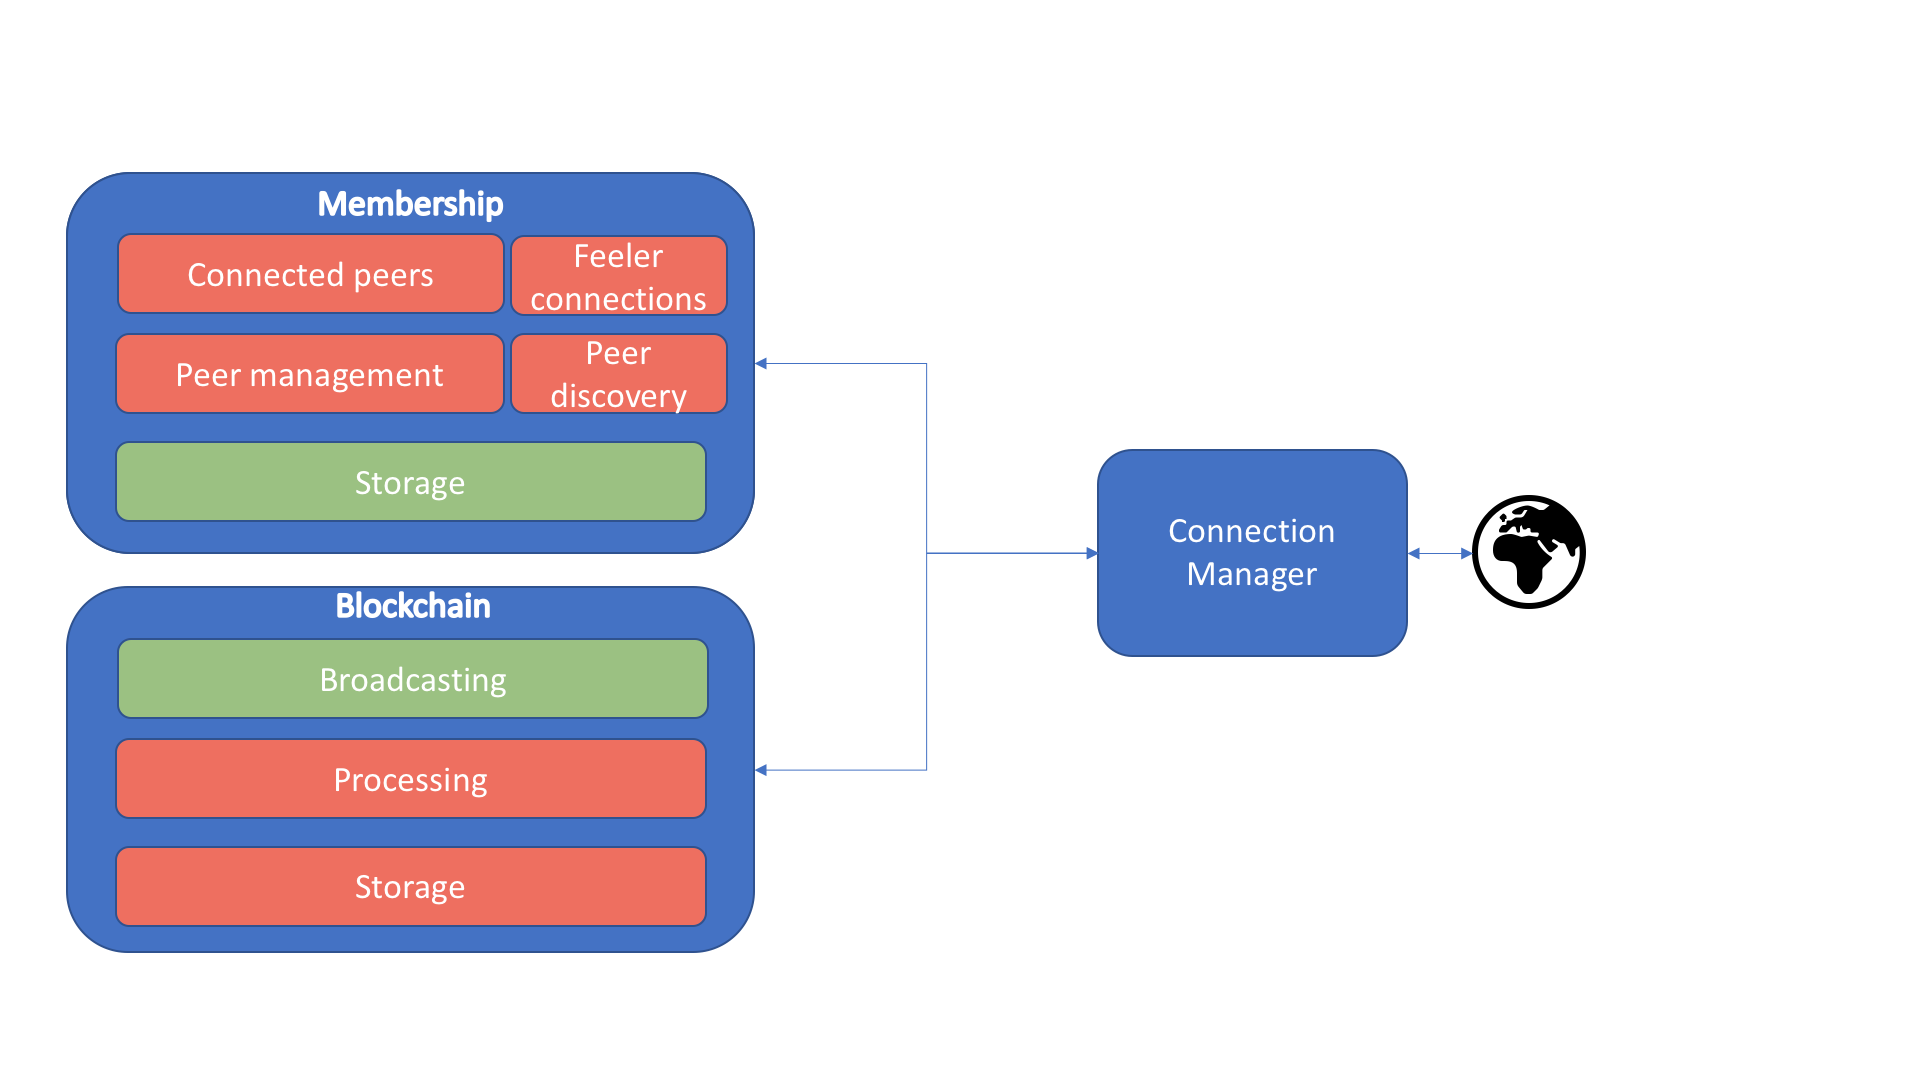
\includegraphics[scale=0.4]{figs/Architecture.png}
\caption{Bitcoin architecture with the modules that we modify highlighted in green}
\label{fig:arch}
\end{figure}


\section{Ranking Neighbours}
\label{sec:ranking}
As miners are only a small fraction of the network, not all nodes will be directly connected to miners.
As previously mentioned, our protocol has the requirement that nodes have to determine from their neighbours which ones are mining blocks.

A simple approach is to simply count the number of hops a block takes since it is created until it reaches a node. 
This means that if a node had a miner \textsl{A} and a miner \textsl{B} at distances 1 and 2 respectively. If for instance, the node received a block created by \textsl{A} then that block would have a field with the distance with value 1. With this information the node would give priority to \textsl{A} when disseminating transactions. 
However, this has two problems. The first is that this is prone to manipulation by Byzantine nodes. The second is that the smallest number of hops does not necessarily mean the fastest path from a node to a miner.

It is important to note that we are not trying to exactly determine which node is going to mine the next block, we just want to determine which nodes have a higher probability of mining a block or from the neighbours of a node which nodes are connected to these nodes. 
Hence, the protocol will attribute a higher rank to neighbours that:
\begin{itemize}
    \item Disseminate blocks as fast as possible - because miners once they mine a block want to disseminate that block as fast as possible in order for the rest of the network to build on top of it;
    \item Disseminates all relevant blocks - because once a miner learns about a new block it starts immediately trying to mine on top of that block hence is in its best interest to also relay that block;
    \item Adds transactions as fast as possible to blocks - because apart from the block reward miners also profit from the taxes imposed on transactions when they are added to blocks.
\end{itemize}

With this intuition, each node is going to prioritise the neighbours that have the fastest paths to miners, or are miners themselves.
This is done in a decentralised fashion but results in fast paths to miners emerging over other paths.
Locally, each node, classifies neighbours as follows:

\begin{equation} \mbox{class}^{T}= (\dfrac{k^{T}}{n^{T}} + a^{T} - n^{T} + \dfrac{y^{T}}{z^{T}}) \end{equation}

where:
\begin{itemize}
  \item \textit{k} it the accumulated time it took to a neighbour to disseminate each block to the node;
  \item \textit{n} is the total number of blocks received by a neighbour;
  \item \textit{a} is the total number of blocks received;
  \item \textit{y} is the accumulated time it took for transactions, sent to a neighbour, to be accepted in a block;
  \item \textit{z} is the total number of transactions sent to a neighbour.
  \item \textsl{T} is time frame that we use to know what transactions to take into account when determining the \textsl{class} of a neighbour
\end{itemize}

Going over each part of the equation, let us start with $\dfrac{k^{T}}{n^{T}}$. This fraction represents the pace at which a neighbour relays blocks to a node, for instance \textsl{P}.
Here the time it takes for a neighbour to relay a block to \textsl{P} is given by the difference between the current time and the last time \textsl{P} received a new block from that neighbour. We add the time it took for \textsl{P} to receive all the blocks mined in $T$ from a neighbour and then divide this value by the amount of blocks received, which gives us an average of time it takes for a neighbour to relay blocks to \textsl{P}.

The second part of this formula is $a^{T} - n^{T}$. This allows the classification to automatically adapt to situations where nodes that generate a block sparingly do not get a good classification indefinitely. Because we are subtracting the total number of blocks received ($a^{T}$) by the total number of blocks received from a neighbour (${n^{T}}$). If for instance, a neighbour \textsl{J} does not have a fast connection to a miner or if \textsl{J} was a miner that stopped mining blocks then \textsl{J} will have lower priority versus other neighbours, since it is not able to reliably relay every block to us.
%In fact, even though the majority of blocks is generated by a small subset of miners, sometimes a random node is able to mine a new block successfully.

Finally, the thirth part of this equation $\dfrac{y^{T}}{z^{T}}$ is used to cope with nodes that might not relay transactions. In this fraction, we divide the sum of the time it took to commit transactions that \textsl{P} sent to a neighbour (\textsl{J}) by the number of transactions that \textsl{P} sent to \textsl{J}. With this, \textsl{P} will get an approximation of the average time that \textsl{J} takes to commit a transaction. However, given the large number of transactions that flow through the network, instead of maintaining timers for all of them, we only maintain a timer every one hundred transactions. This prevents overloading nodes with metadata while still giving a good sample of the general network behaviour.

With this in mind, a neighbour has a good classification if: i) it has a good ratio of \textsl{time it takes to disseminate blocks/number of blocks we received from him}, ii) a good ratio of \textsl{blocks received from him/blocks received} and finally iii) a good ratio of \textsl{time it took for a transaction to be added to blocks if we sent it to him}.

Given that the classification of neighbours is prone to change over time, the actual value used to order neighbours is given by the following sliding average of the classification presented previously:

\begin{equation} \mbox{class}^t = (1-\alpha) \cdot \mbox{class}^{t-1} + \alpha \cdot \mbox{class}^{T} \end{equation}

The $\alpha$ factor exists to avoid nodes that generated a lot of blocks in the past but no longer do, from having a good classification forever and to prevent very dramatic fluctuations in the classifications of neighbours. In our experiments, we used an $\alpha=0.3$ and a \textit{T} configured to be an interval of four hours. We used a $\alpha=0.3$ because we wanted to give more importance to that the past of a node than to the present as sometimes nodes might disconnect from that network or might not have the luck to mine a block in a longer time period. We also tried with other values of $\alpha$, but we found 0.3 to give us the best results. Regarding the four hours of interval, we also tried multiple values and we obtained better results with the interval being four hours.

\begin{algorithm}
\begin{algorithmic}[1]
\Function{update\_nodes\_classification}{$node\_to\_update$}
\State $scores \gets \textsl{[ ]}$
\For{$node$ \textbf{in} $neighbourhood$}
  \State $score \gets get\_classification(node)$
  \State $scores.append([score, id])$
\EndFor
\State $sort(scores)$ \textit{// sort by score from lower to higher}
\State $top\_nodes \gets \textsl{[ ]}$
\For{$i$ \textbf{in} $range(0, max\_t\_nodes)$}
  \State $top\_nodes.append(score[i][1])$
\EndFor
\EndFunction
\end{algorithmic}
\caption{Top neighbours computation}
\label{alg:class}
\end{algorithm}

Hence in our protocol, each time a node receives a block from a neighbour the classification of the neighbours will be updated using Algorithm~\ref{alg:class}. The node will iterate over his neighbours and for each one, it will calculate his classification using Equation~3.3 and then it will append his classification together with his ID to a vector named scores (lines 3 to 6). After that, the node sorts the scores vector from the lowest score to the highest score, this means the nodes with the lowest score will be closest to the index 0 of the vector (line 7). Finally, the node will iterate from 0 to the max number of top nodes and append the first $max\_t\_nodes$ of the vector of \textsl{top nodes} (lines 9 to 11). The values for the variable $max\_t\_nodes$ will be discussed in the next section.

In the end, the node will have in its list of \textsl{top\_nodes} the set of nodes with the lowest classification. Note that a low classification means that a node has a good/fast connection to at least a miner or a neighbour of a miner meaning the lower classification the better is that connection.

\section{Skewed Relay}
\label{sec:sr}
%Given that our objective is that transactions reach a miner as fast as possible, we can use the mechanism described previously to do it.

If all nodes followed the protocol and did not crashed or leaved the network, it would suffice to use the mechanism described above with the variable $max\_top\_nodes = 1$ to send
%Hence, if all the nodes were to follow the protocol correctly, and the paths created by out solution were resilient enough we could send our
transactions to only one node, as we would be sending the transactions to the best neighbour of each node which would eventually make the transactions appear in a block. With this we would also be lowering the amount of duplicated advertisements from 6.6 to 1.

However, even if we do not consider the problem of node failure and Byzantine behaviour, there is the problem of commit time. Commit time for cryptocurrencies is very important as not only a low commit protects the system against some attacks but also makes the cryptocurrency more appealing as transactions become confirmed faster.
As mentioned previously, the variance of the mining process could result in a prolific miner not being able to successfully mine a block for an extended period of time, precluding transactions sent exclusively to it from being included in the blockchain which could make multiple nodes vulnerable to the double-spending attack. Furthermore it is not guaranteed which node is going to mine the next block hence, it is unadvised to send all the transactions of a node to only one neighbour.

\begin{algorithm}
\begin{algorithmic}[1]
\Function{nodes\_to\_send}{$tx$}
\If{$(ip == True$ \textbf{and} $tx.source() == self)$}
	\State {$\textbf{return}$ $neighbours$}
\EndIf
\State $total \gets max\_t\_nodes + max\_r\_nodes$
\If{$size(neighbours) < total$}
	\State $total \gets size(neighbours) - max\_t\_nodes$
\Else
	\State $total \gets total - max\_t\_nodes$
    \EndIf
\If{$total > 0$}
	\State $r\_nodes \gets rand\_choice(neighbours, total)$
    \EndIf
\State \Return $t\_nodes + r\_nodes$
\EndFunction
\end{algorithmic}
\caption{Nodes to send transactions advertisements computation}
\label{alg:diss}
\end{algorithm}

We address this - and simultaneously node failures and Byzantine behaviour - by sending transactions not only to the \textsl{t} top nodes but also to \textsl{r} random nodes, as described in Algorithm~\ref{alg:diss}. The variable \textsl{\acrshort{ip}} (\acrlong{ip}) indicates that if a transaction is generated by a node, the node has the option of either sending it to \textit{t} plus \textit{r} neighbours or to all of them. We implemented this feature to be able to understand if the first relay had much impact in the commit time of a transaction.

Hence, every time that a node has to relay a transaction it will start by verifying if the variable \textsl{\acrshort{ip}} is enabled or not if it is it will return the full neighbourhood similar to Bitcoin (lines 2 to 4). If it is not then the node will start by adding the values of $max\_t\_nodes$ and $max\_r\_nodes$ to simply check if the size of the neighbourhood of the node is big enough to cope with the value of both variables added. In the end, the node will have in the variable $total$ the number of nodes not in $top\_nodes$ that can potentially be chosen as random nodes (lines 5 to 10). With this, the node will then randomly choose $total$ nodes from the set neighbourhood excluding the nodes in $top\_nodes$ (line 11 to 13), in the end, this algorithm will return both sets.

This way we ensure that transactions reach the nodes with the higher probability of mining a block but also reach the rest of the network. Hence, ensuring that not only the transactions are committed in a timely manner but also reach other nodes lowering the probability of those nodes being attacked.

This dissemination process can then be configured with the following variables: \textsl{max\_t\_nodes}, \textsl{max\_r\_nodes} and \acrshort{ip} to obtain different results in the information dissemination.
We study the impact of these parameters more in depth in Section~\ref{sec:sri}.

\section{Adapting to Network Changes}
\label{sec:nc}
A key aspect of \acrlong{p2p} networks is that nodes can leave or join the network at any  time. With this in mind, we designed an algorithm that adapts to the network in order to keep the commit time of the transactions while still trying to send as few messages as possible. 

Hence, we designed an algorithm that starts by attributing a value of $size(neighbourhood) / 2$ to both \textsl{max\_t\_nodes} and \textsl{max\_r\_nodes} simulating the Bitcoin dissemination process. Then each node monitors the commit time of its transactions, if this commit goes over or below a specified threshold the node is going to either increase or decrease the values of both \textsl{max\_t\_nodes} and \textsl{max\_r\_nodes} by one. With this end up with an algorithm that can behave in the worst case like Bitcoin and in the best case can bring improvements to the current protocol.

\begin{algorithm}
\begin{algorithmic}[1]
\Variables
 \State $TIME\_TX\_CONFIRM \gets 30*60$ // Maximum time allowed for a transaction to be committed
 \State $TIME\_TO\_WAIT \gets 4*60*60$ // Time to wait before the node is able to increase or decrease max\_t\_nodes and max\_r\_nodes
\EndVariables
\Function{increase\_relay}{\null}
\State $now \gets get\_current\_time()$
\State $avg\_time \gets get\_avg\_time\_unconfirmed()$
\State $timeout \gets avg\_time > TIME\_TX\_CONFIRM$
\State $space \gets max\_t\_nodes + 1 \leq neighbourhood / 2$
\State $cooldown \gets last\_inc + TIME\_TO\_WAIT \leq now$
\If{$timeout$ \textbf{and} $space$ \textbf{and} $cooldown$}
  \State $increase(t, r, 1)$ // increase by one both max\_t\_nodes and max\_r\_nodes
  \State $had\_to\_inc \gets True$
  \State $UPDATE\_NODES\_CLASSIFICATION()$
  \State $last\_inc = now$
  \State $relay\_delayed\_TX()$
\EndIf
\State $cooldown \gets last\_dec + TIME\_TO\_WAIT \leq now$
\If{\textbf{not} $had\_to\_inc$ \textbf{and} $cooldown$}
  \State $avg\_time \gets get\_avg\_time\_confirmed()$
  \State $timeout \gets avg\_time <= TIME\_TX\_CONFIRM$
  \State $space \gets max\_t\_nodes - 1 \leq 0$
  \If{$timeout$ \textbf{and} $space$}
    \State $decrease(t, r, 1)$ // decrease by one both max\_t\_nodes and max\_r\_nodes
    \State $UPDATE\_NODES\_CLASSIFICATION()$
    \State $last\_dec = now$
  \EndIf
\EndIf
\EndFunction
\end{algorithmic}
\caption{Adaptive dissemination}
\label{alg:inc}
\end{algorithm}

%As  depicted in Algorithm~\ref{alg:inc}, we automatically adjust the values of \textsl{max\_t\_nodes} and \textsl{max\_r\_nodes} depending on whether the node's transactions are taking too long to be committed or are being committed in a  timely fashion.

%Briefly, if the current average of the time it takes for the unconfirmed transactions of a node to be committed to a block, gets bigger than the constant \textsl{TIME\_TX\_CONFIRM} (30 minutes) then the node is going to increase both the size of \textsl{max\_t\_nodes} and \textsl{max\_r\_nodes}, and relay the transactions that took more than 30 minutes to commit.

%If the average of all unconfirmed transactions does not surpass the threshold of the 30 minutes, the node will check if the average time it took to commit its confirmed transactions in the last hour took less than \textsl{TIME\_TX\_CONFIRM}. If so the node will lower the size of \textsl{max\_t\_nodes} and \textsl{max\_r\_nodes} by one, otherwise it will not do anything.

With this, each node is going to invoke Algorithm~\ref{alg:inc} every ten minutes as that is the average rate which blocks are mined. The algorithm starts by assigning to $avg\_time$ the average time its unconfirmed transactions are taking to be accepted (line 3). The time that is taking for an unconfirmed transaction to be confirmed is calculated by subtracting the current time with the time of creation of said transaction. Then the node will check if $avg\_time$ is bigger than the constant \textsl{TIME\_TX\_CONFIRM} (30 minutes). 

If it is, this means the node will check if it can increase the values of both \textsl{max\_t\_nodes} and \textsl{max\_r\_nodes}, if it can then is going to increase both and relay the transactions that took more than 30 minutes to commit (lines 4 to 13).

If the average of all unconfirmed transactions does not surpass the threshold of the 30 minutes, then the node will first check if the average time it took to commit its confirmed transactions in the last hour took less than \textsl{TIME\_TX\_CONFIRM} (lines 14 to 15). If so the node will check if it can lower the values of \textsl{max\_t\_nodes} and \textsl{max\_r\_nodes} by one, if yes it will do it otherwise it will not do anything (lines 16 to 23). 

We have chosen the threshold to be 30 minutes as that is the highest time registered in \url{blockchain.info} for transactions to be committed. We also have chosen to increase/decrease always both variables because as we are going to see in the next chapter when we run our protocol with $max\_r\_nodes = 0$ we did not obtain the best results, this way we make sure that both values will never be lower than 1. We also have chosen to only increase/decrease both values by one because we have also noticed that little changes like sending transactions to only one fewer neighbour already had a great impact.

Regarding the variables $cooldown$ (lines 6 and 14) in the algorithm they are used because each time \textsl{max\_t\_nodes} and \textsl{max\_r\_nodes} are changed the node will not be able to change these values in the next 2 hours to prevent fluctuations in these values. Furthermore, every time a node increases \textsl{max\_t\_nodes} and \textsl{max\_r\_nodes} it will not be able to decrease these values in the next 4 hours in order to prioritise resilience over performance. 


\section{Implementation}
\label{sec:imp}

To evaluate our proposal we have resorted to simulations, given that it would have been impossible to setup a realistic experiment with large number of users in the timeframe available to complete this work. Unfortunately, although a number of Bitcoin simulators have been proposed in the past, they are no longer supported and, furthermore, they implement algorithms that do not match the current version of Bitcoin. Therefore, we have opted to implement our own simulator. In order to collect data useful to calibrate the simulator, we have also created a modified version of the standard Bitcoin client that has been enriched with a number of probes to collect statistics about the Bitcoin operation.

In this section, we start by describing the modification we did to the Bitcoin client to collect statistics and then we describe our simulator.

%To develop and implement our approach we had to go through multiple challenges, from properly understanding how Bitcoin works to implementing the Bitcoin broadcast protocol in an event driven simulator to test our approach.

%In this section, we will go over two crucial points of our work apart from the ones already described. We will start by covering how we modified the Bitcoin client to gather more information about the system and then we will go into how we implemented the Bitcoin broadcast protocol in an event driven simulator.

\subsection{Modifying the Bitcoin Client}

As we will describe in the next section, we opted to build a new simulator, that runs the most recent version of the Bitcoin protocols. In order to ensure that the simulator accurately captures the behaviour of the real system, we need to collect a number of statistics regarding the operation of the Bitcoin network such as:

\begin{itemize}
    \item Percentage of duplicated advertisements;
    \item Percentage of transactions that needed to be requested;
    \item Percentage of duplicated blocks received;
    \item Percentage of blocks received by neighbour;
    \item Percentage of blocks where a node needed to request transactions
\end{itemize}

Although there are a few websites, such as \url{blochain.info} and \url{bitnodes.earn.com}, that publish some information regarding the operation of the Bitcoin network, these sites do not offer the level of detail required to calibrate the simulator.  Therefore, we opted to create a modified version of the Bitcoin client, that was augmented with a number of sensors to collect the following information:

\begin{itemize}
    \item Blocks received - hash, source, message type
    \item Advertisements for transactions - hash, source
    \item Transactions received - hash, source
    \item Transactions requested with \textsl{GetBlockTX} - hash, block hash
\end{itemize}

After studying the sources of the Bitcoin distribution, we did realise that it was possible to implement most of these sensor by introducing small changes to the \textsl{net\_processing.cpp} file of the Bitcoin distribution (this file includes most of the logic associated the the Bitcoin broadcast protocol).

In order to collect the desired statistics, we have deployed to instances of the modified client connect to two different services providers (one using the academic network and another using one of the main Portuguese internet providers). We have ensured that the two clients did not establish a connection between them as that would skew the results. We have collected the statistics by running the two modified clients for more than one month, after discarding the results collected during an initial warm-up period of 7 days.

%In order to understand the Bitcoin system more in-depth we started by not only studying the source code, as the available documentation was and still is very poor for new developers, but also we made some modifications to the Bitcoin core client in order to collect important metrics. 

%To be able to do these modifications we had to understand properly how the Bitcoin code was structured as this system is composed by more than 60 files were some of them have more than 3000 lines of code that are modified on a daily basis. For a new developer, the absence of any guidance when confronted with this project can be quite overwhelming. Hence, we had to start searching keywords to be able to find where were the chunks of code that were interesting to us. After some time with the code, we then understood that the main file that interested us was the net\_processing.cpp where a lot of the logic of broadcasting protocol was present. After this exercise collecting the metrics that we wanted was much more simple we only had to understand how the structures of the system were implemented to be able to extract the information that we wanted and write it to some a file. 

%In the modifications that we made we modified the client so it would log all the following metrics:
%\begin{itemize}
%    \item Blocks received - hash, source, message type
%    \item Advertisements for transactions - hash, source
%    \item Transactions received - hash, source
%    \item Transactions requested with \textsl{GetBlockTX} - hash, block hash
%\end{itemize}

%We wanted to collect these specific metrics for two main reasons, first, we needed them to understand if some of our ideas to improve the protocol would have an impact. The second reason is that although the metrics available on websites like \url{blochain.info and bitnodes.earn.com} are useful they do not tell us the full picture of the system which we can only obtain if we make a more fine-grained evaluation of the system and the messages exchanged by the peers in this system.

%With the modified Bitcoin we deployed two clients in two different machines which were geographically close. However, we guaranteed that both machines never establish a connection between them as that would skew the results obtained. A client was deployed in INESC-ID and the other was deployed in a house in Benfica. Both clients ran at least over a period of a month and we discarded any information collected in the first days to observe the system in a stable state.

%We then analysed this metrics to extract multiple statistics like the following:
%\begin{itemize}
%    \item Percentage of duplicated advertisements;
%    \item Percentage of transactions that needed to be requested;
%    \item Percentage of duplicated blocks received;
%    \item Percentage of blocks received by neighbour;
%    \item Percentage of blocks where a node needed to request transactions
%\end{itemize}
%
%With these metrics and a good understanding of the systems, we were able to develop and perfect the protocol presented in this thesis.

\subsection{Implementing the Simulator}

To the best of our knowledge, when we started this work, two Bitcoin simulators were available, namely \url{https://github.com/shadow/shadow-plugin-bitcoin} and \url{https://github.com/arthurgervais/Bitcoin-Simulator}. Unfortunately, these simulators did not implement the latest versions of Bitcoin, namely they did not simulate the use of compacts blocks. Furthermore, the simulators were no longer supported. Finally, these simulators include many mechanisms that are irrelevant to evaluate our contributions. Instead of attempting to update these simulators, we opted to implement our own simulator, that would be focused on simulation the aspects of Bitcoin that we aim at improving with our algorithm.

Our simulator is an event driven simulator, where the behaviour of each node is described by a deterministic state machine, that consumes events and, in response, produces events. Each event is tagged with a \textit{timestamp}, that captures at which instant the event should occur, and a \textit{target}, that specifies the node that should process the event. For instance, if a node $n_1$ receives an event $e_1$ at time $t$, and this event represents an message that needs to be relayed immediately to node $n_2$, the  processing of event $e_1$ would generate another event $e_2$ targeted at node $n_2$ and scheduled to occur at time $t+\delta$, where $\delta$ is a function of the network latency between $n_1$ and $n_2$. The simulator was coded in Python2.7.

The simulator allows the user to configure a number of Bitcoin network parameters such as the number of nodes, the initial neighbourhood size of nodes and the number of miners. Based on these configuration parameters, the simulator automatically assigns an initial view of 8 neighbours to each node. The duration of a simulation is measured by the number of cycles that each node will perform; in or implementation one cycle is equal to one second. In each cycle, each node checks the following i) if it needs to run Algorithm~\ref{alg:inc}, ii) if it should generate a new transaction, iii) if it should generate a block, and iv) finally if it should send any messages to any of its neighbours. As noted in Section~\ref{sec:sm}, the simulation is configured to generate blocks at a rate of 1 block per 10 minutes and 2 transactions per second, in order to obtain 172 800 transactions per day (which is the average number of transactions per day registered in Bitcoin at the time of this writing). 

It is worth noting that the current version of the simulation was the result of multiple iterations, namely because earlier version did not optimise the memory usage and, therefore, could not run simulation with very large numbers of nodes. We omit the description of these code optimisation's as they are orthogonal to the main contribution of the thesis.

%While we were studying the Bitcoin code we also were thinking of how we would test our ideas and prototypes. We started by trying to use a simulator that we have found when we were writing the project for our thesis. However, this simulator was not working and it had stopped being updated a long time ago, we also tried to search for other simulators but they were either not working or they did not implement the latest versions of Bitcoin, namely compacts blocks~\footnote{Some examples \url{https://github.com/shadow/shadow-plugin-bitcoin} and \url{https://github.com/arthurgervais/Bitcoin-Simulator}}. Implementing our ideas and prototypes in the Bitcoin client and use that for testing was also an idea out of the question. Since not only some early prototypes of our protocol modified the core structure of Blocks but also it would take a lot of time to implement a single prototype given at the time our understanding of the Bitcoin source code. Hence, we decided to implement the Bitcoin broadcast protocol in an event driven simulator to test our approach.

%Implementing the protocol itself was probably what took us more time to do as not only we had to thoroughly go over the code to make sure we did not miss any important functionality, but we also had to always think of what functionality was important and could have an impact on the results. 

%We implemented the protocol in a simulator coded in Python2.7, we will now give an overview of how the protocol was implemented, we will not go much in depth in this explanation as much of the behaviour implemented was already described in Section~\ref{sec:bb}. 

%In our implementation, before the simulation stars, we will assign a couple of values to some important variables like the number of nodes, the initial neighbourhood size of nodes and the number of miners. Each node is also initialised with the necessary data structures and a list with his initial 8 neighbours.

%After initialisation, the simulation starts, the duration of a simulation is measured by the number of cycles that each node will have to perform, in or implementation one cycle is equal to one second, as some behaviour was only captured if we simulated time equal to seconds.

%In each cycle, each node will have to verify if it is time to run Algorithm~\ref{alg:inc}, if it should generate a transaction if it should generate a block and finally if it should send any messages to any of its neighbours. As we have mentioned in our system model Section~\ref{sec:sm} we configured our implementation to generate blocks at a rate of 1 block per 10 minutes and 2 transactions per second to obtain 172 800 transactions a day which is the average registered in Bitcoin. 

%The rest of the implementation is for the majority quite straightforward, we decided to implement the protocol using a top-down approach where we started by implementing all the messages types and only after did we implement more specific behaviour to each message type. For a more detailed implementation, the reader can also visit the GitHub of the project at \url{https://github.com/JoaoBraveCoding/bitcoin-simulator}.

%Finally, another interesting challenge worth mentioning was the management of memory that we needed to perform multiple times to run our simulations. As we will describe more in-depth in Section~\ref{sec:sim_tuning} we had problems running simulations with the size of the Bitcoin network that we registered at the of our experiments.

%The main cause of this problems was the number of transactions created, as 2 transactions are created each cycle and in the base protocol each node will relay those transactions to all their neighbours is easy to understand that the amount of information to be processed is going to grow exponentially. Furthermore, the programming language that we used was also not the best for this kind of protocol implementation as Python is not know by his high performance. Because of this, we had to perform multiple patches to the simulator each time we modified it in order to achieve a balance between the memory/CPU consumed and the size of the network. We had to change multiple data structures and evaluate which ones would give us a better trade-off.

\section{Summary}
\label{sec:wsum}
This chapter presented a new transaction dissemination protocol that aims at reducing the amount of resources used by the Bitcoin network while still maintaining the resilience of the system. In order to do so, a new algorithm to rank neighbours was developed as well as an algorithm to bias the dissemination of transactions in the Bitcoin network. Furthermore, we also developed an algorithm that allows the dissemination protocol to adapt itself, in response  to changes in the network. 
%Finally, we also implemented the Bitcoin protocol in an event simulator to test our novel protocol.